\chapter{SafeWatch: Sistema de Detecção de Quedas}
\label{cap:safeWatch}

Um evento de queda pode ser bastante prejudicial a saúde do indíviduo, pricipalmente de um idoso. Pensando nisso, diversos tipos sistemas de detecção de quedas foram desenvolvidos. Neste trabalho, apresentamos o SafeWatch, uma solução integrada entre smartphone e smartwatch, onde quedas são detectadas de maneira automatizada, e se necessário, os contatos de emergência do idoso são informados de sua localização para que se possa prestar socorro de forma mais rápida possível. 


As seções desse capítulo são organizadas da seguinte maneira: A seção \ref{sec:architecture} mostra a arquitetura que foi definida e utilizada pela ferramenta construída; A Seção \ref{sec:tools} mostra as ferramentas que foram utilizadas para auxiliar a construção do SafeWatch; A Seção \ref{sec:implementation} descreve detalhes da implementação do SafeWatch; Por fim, a seção \ref{sec:screens} ilustra a execução da ferramenta.



\section{Arquitetura}
\label{sec:architecture}

De acordo com \cite{garlan1993introduction}, a arquitetura de um software define o sistema em termos de componentes e as interações existentes entre esses componentes. Em outras palavras, a arquitetura de software tem o objetivo de mostrar uma visão completa do sistema. 

O SafeWatch foi desenvolvido para funcionar como um aplicativo Android Wear\footnote{https://www.android.com/wear/} para smartwatches que funciona em conjunto com o smartphone Android do usuário, atravês de uma aplicação homônima, que está sincronizado com o mesmo. A ferramenta foi desenvolvida com base em uma arquitetura pré-definida e possui os seus módulos desacoplados para facilitar futuras mudanças ou melhorias. A ferramenta está dividida em 5 módulos como ilustra a figura \ref{fig:architecture}.

\begin{figure}[ht]
	\centering
	\includegraphics[scale=0.65]{imagens/architecture.png}
	\caption{ Arquitetura do SafeWatch. Figura Elaborada pelo autor (2016).}
	\label{fig:architecture}
\end{figure} 



\begin{itemize}
	\item{\textbf{Sensor Reader (Parte 1 da figura \ref{fig:architecture})}: Responsável pela configuração e gerenciamento dos sensores, mais especificamente do único sensor utilizado, o acelerômetro. }
	
	\item{\textbf{Fall Detector (Parte 2 da figura \ref{fig:architecture})}: Recebe informações provindas do \textit{Sensor Reader} para através do algoritmo de detecção de quedas categorizar um determinado evento como queda ou não.}.
	
	\item{\textbf{Watch Communicator (Parte 3 da figura \ref{fig:architecture})}: Realizará a comunicação entre o smartwatch e o smartphone do usuário. Irá receber dados do smartwatch que são tratados pela módulo chamado de \textit{Fall Handler}.}
	
	\item{\textbf{Fall Handler (Parte 4 da figura \ref{fig:architecture})}: Será responsável pelas ações do smartphone após um evento de queda, como o envio de emails e o gerenciamento dos dados do acelerômetro recebidos do smartwatch.}
	
	\item{\textbf{Contact Manager (Parte 5 da figura \ref{fig:architecture})}: Será responsável pelas gereciamento dos contatos de emergência do usuário. Ações como visualização, adição e remoção de contatos estão encapsuladas neste módulo.}
			
\end{itemize}

Os módulos \textit{Sensor Reader} e \textit{Fall Detector} estão presentes na aplicação embarcada no smartwatch, os demais módulos estão presentes na aplicação para smartphones. 

\section{Ferramentas Utilizadas}
\label{sec:tools}
Durante o desenvolvimento do \textit{SafeWatch} foram utilizadas diversas ferramentas que serviram para dar suporte a sua implementação e execução. Tanto o aplicativo para smartphones, quanto o aplicativo embarcado no smartwatch foram desenvoldidos utilizando o Android Studio\footnote{https://developer.android.com/studio/}. O Android Studio é a \ac{IDE} oficial do Google no desenvolvimento de aplicações móveis ou vestíveis. 


Nas classes do projeto relacionadas as telas do aplicativo foi utilizado o ButterKnife\footnote{texthttps://github.com/JakeWharton/butterknife}. O Butterknife é responsável por fazer a ligação entre os arquivos responsáveis pela criação das telas, e as classes que utilizam os componentes visuais destas telas. 

Para realizar os cálculos do desvio padrão foi utilizada a biblioteca do Apache chamada Commons-Math\footnote{http://commons.apache.org/proper/commons-math/}. Este biblioteca contém um conjunto de funções matemáticas e de estatística não presentes na biblioteca padrão do JAVA. 

Para que possamos enviar os dados do acelerômetro do smartwatch para o smartphone, eles precisam estar codificados em algum padrão, o padrão escolhido foi o JSON. O JSON é um formato de dados utilizado para comunicação entre dispositivos \citep{JSON;16}. Para que possamos fazer a codificação e decodificação dos dados do acelerômetro foi utilizado a biblioteca chamada Gson\footnote{http://www.json.org/}.

Por fim, para o envio de emails para os contatos de emergência foi utilizado as biblioteca padrão criada pela Oracle\footnote{http://www.oracle.com/} chamada de JavaMail\footnote{http://www.oracle.com/technetwork/java/javamail/index.html}. 





\section{Implementação}
\label{sec:implementation}
A implementação do SafeWatch foi dividida em várias partes, onde cada um delas é representada por um módulo independente dos demais. A linguagem de programação utilizada foi Java\footnote{http://www.oracle.com/technetwork/java/index.html}, linguagem padrão no desenvolvimento de aplicações Android. Nas seções abaixo são detalhados detalhes da implementação e funcionamento de cada módulo.


\subsection{Sensor Reader}
O módulo \textit{Sensor Reader} é responsável pela configuração e gerenciamento do acelerômetro. Aqui, o acelerômetro é configurado para atualizar seus dados a um frequência de 50 $Hz$, ou seja, a cada 20 ms. Os dados do acelerômetro são coletados a todo momento, mesmo quando a aplicação não está em primeiro plano.

Este módulo também será responsável por armazenar os dados do acelerômetro nos últimos 0.4 segundos para posterior uso no algoritmo de detecção, caso necessário. Tanto a escolha da frequência de 50 $Hz$ quanto o tempo de 0.4 segundos para o armazenamento de dados do acelerômetro serão explicados com mais detalhes em \ref{subsec:fall_detector}.



\subsection{Fall Detector}
\label{subsec:fall_detector}
O módulo \textit{Fall Detector} encapsula o algoritmo de detecção de quedas baseado em limiares utilizado pelo SafeWatch. Este é o módulo mais complexo da aplicação, pois nele se encontra a lógica responsável por decidir, através dos dados obtidos do acelerômetro, se um evento de queda ocorreu ou não. O algoritmo proposto é uma adaptação do algoritmo desenvolvido por \cite{hsieh2014wrist}. O algoritmo proposto neste trabalho se diferencia do algoritmo proposto em \cite{hsieh2014wrist} pela não utilização do giroscópio como sensor auxiliar, acredita-se que sem o uso do giroscópio é possível obter-se resultados satisfatórios como visto em \ref{subsec:F2D_System}. 

Um grande desafio quando utilizamos um algoritmo baseado em limiares é a definição dos valores dos limiares. Caso este valor seja muito alto, o sistema irá deixar escapar alguns eventos de queda, mas não irá categorizar uma \ac{ADL} como uma queda.  Do outro lado, se este valor for muito baixo, o sistema irá detectar todos os eventos de queda, mas algumas \ac{ADL} pode ser categorizadas como eventos de queda de maneira equivocada. De acordo com o treinamento inicial realizado por \cite{hsieh2014wrist}, o valor de \ac{SMV}, representado pela fórmula \ref{eq:SMV}, será maior que $6G$, onde $G \approx 9.8 m/s^2$,  no momento do impacto em um evento de queda. 

Também foi identificado por \cite{hsieh2014wrist}, que caso o valor de aceleração atinja o valor de $6G$, o valor do desvio padrão ficava com valores em torno de $1.07G$  em movimento regulares do braço realizados 0.4 segundos antes ou depois deste pico de aceleração.Entretanto, em eventos de queda este valor estava mais próximo de $1.69G$. 

Por fim, o periodo de inatividade posterior a uma queda foi analisado. De acordo com \cite{hsieh2014wrist}, o valor da \ac{SMA}, expresso atráves da equação \ref{eq:SMA}, tem uma relação diretamente proporcional com o nível de movimentação de um corpo. Foi identificado que em eventos de queda, o indíviduo tende a ficar parado por pelo menos 2 segundos, com valores de SMA inferiores a $200G$. E importante resaltar que este valor de $200G$ é encontrado quando a frequência do acelerômetro é de 50 $Hz$.Caso contrário, o número de amostras coletados será diferente, afetando diretamente no valor de $SMA$. 

\begin{equation}
SMA = \sum_{i=1}^{N} (\mid X_i\mid + \mid Y_i \mid + \mid Zi_i \mid)
\label{eq:SMA}
\end{equation}

Nesta equação $X_i$, $Y_i$, $Z_i$, são os valores da aceleração no tempo $i$ e $N$ é o número de amostras desejadas. Levando como base o treinamento inicial descrito acima foi possível desenvolver o algoritmo descrito na imagem \ref{fig:flow_chart}.

\begin{figure}[ht]
	\centering
	\includegraphics[scale=0.75]{imagens/flowChartAlgorithm.png}
	\caption{ Fluxograma do algoritmo proposto. Figura Elaborada pelo autor (2016).}
	\label{fig:flow_chart}
\end{figure} 

	\begin{enumerate}
		\item Os valores do acelerômetro são monitorados, caso $SMV$ seja maior do que $6G$, os demais valores de $SMV$ são monitorados por mais 0.4 segundos. O maior dos valores observado neste tempo é marcado como pico de aceleração e o algoritmo prossegue para o passo 2.
		\item O desvio padrão de \textit{SMV} é calculado, nos 0.4 segundos anteriores e posteriores a detecção do maior valor de SMV. Caso este valor não seja menor do que $1.5G$,  o algoritmo irá para o passo 3.
		\item O valor de $SMA$ é calculado, e caso este valor seja menor do que $ 200G $ finalmente confirmamos que um evento de queda ocorreu.
	\end{enumerate}

 Caso um evento de queda seja detectado, o relógio irá vibrar por 15 segundos, na espera de um feedback do usuário informando se ele está bem ou não. 

\subsection{Watch Communicator}
O módulo \textit{Watch Communicator} é responsável pela comunicação entre o smartwatch é o smartphone do usuário. Fisicamente, está comunicação é realizada via bluetooth, já a nível de software está comunicação é realizada através do que chamamos na arquiterura Android de \textit{Services}.

No Android, um \textit{Service} é um componente da aplicação capaz de realizar operações de longa duração em background e não provém uma interface com o usuário \cite{servicesAndroidDocs}. No SafeWatch os \textit{Services} recebem os dados do acelerômetro referentes ao evento de queda, ou seja todos os registros do acelerômetro 0.4 segundos antes do pico de aceleração, até 2 segundos depois deste valor. Além disso, também é enviado, uma variável booleana indicando se devemos ou não enviar um e-mail para a lista de contatos de emergência do usuário. Os emails de emergência são enviados para a lista de contato do usuário 15 segundos após um evento de queda, ou antes disso, caso o usuário confirme que precisa de ajuda. 

Para que os contatos da lista de emergência não sejam incomodados desnecessariamente na ocorrência de falsas detecções de quedas, o usuário poderá cancelar o envio dos emails de emergência, dentro de 15 segundos após um evento de queda, caso ele informe que está bem.

\subsection{Fall Handler} 
Este módulo é responsável pelo envio de e-mails e a manipulação de arquivos com os dados de uma queda. Para que se possa realizar o envio de e-mails, foi criado um email padrão do SafeWatch através do Gmail\footnote{https://mail.google.com}. O envio de e-mail é feito de forma assincrona, sem bloquear a interação do usuário com a aplicação. 

Os dados referentes a um evento de queda são salvos na raiz do sistema de arquivos do smartphone android na pasta \textit{/SafeWatch/smartwatch}. O arquivo é nomeado com o padrão \textit{experimentData\_timeStamp}, onde t\textit{timeStamp} representa o momento do salvamento do arquivo, em milisegundos. O arquivo está salvo no formato \textit{CSV}, com os valores de aceleração nos eixos x,y,z, o valor de \ac{SMV} correspondente ao registro e o tempo em milisegundos em que ele ocorreu. Apesar destes valores não serem de grande uso para o usuário final, ele poderão servir para o aprimoramento do aplicativo através da análise dados para verificação de limiares. 

\subsection{Contact Manager}
Neste módulo estão encapsulados as ações de adição, remoção e listagem dos contatos de emergência do usuário. Além do e-mail, nas informações do contato também constará o nome completo do mesmo. 


\section{Telas e Funcionamento}
\label{sec:screens}
O SafeWatch foi desenvolvido para funcionar como uma aplicativo android, atravês de uma solução integrada entre smartphone e smartwatch. O sistema foi desenvolvido de forma que o usuário necessite interagir o mínimo possível com os aplicativos tanto no smartphone quanto no smartwatch. 

De forma geral, a aplicação smartwatch irá monitorar as atividades do usuário através do acelerômetro e no momento que uma queda for detectada emitirá um alerta vibratório juntamente com um sinal para o smartphone. No smartphone está presente uma aplicação de gerenciamento geral do sistema, nesta aplicação o usuário será capaz de adicionar, visualizar e remover os contatos de emergência que seriam notificados no momento de uma queda.

Inicialmente, o usuário deve realizar o cadastro dos contatos de emergência, a tela de cadastro pode ser vista na figura \ref{fig:add_contact}. O usuário necessita informar o nome completo e email do contato desejado. Todos os contatos de emergência do usuário podem ser visualizados em forma de lista como pode ser visto na figura \ref{fig:list_contacts}.


Depois de adicionar os contatos de emergência, o usuário não necessita realizar mais nenhum tipo de cadastro ou configuração no sistema. Na ocorrência de uma queda o sistema irá se comportar como pode ser visto na figura \ref{fig:diagram}.


\begin{figure}[ht]
	\centering
	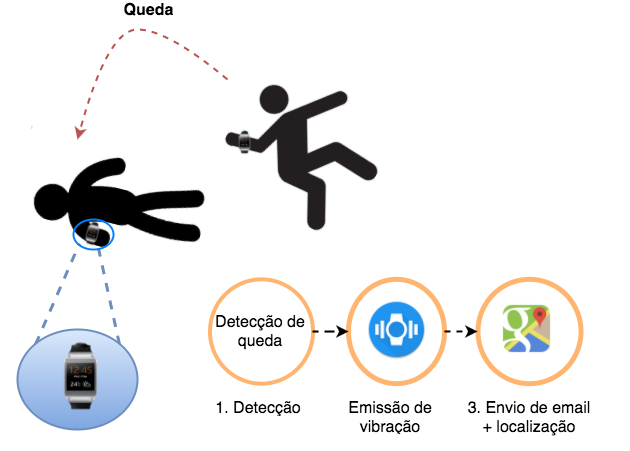
\includegraphics[scale=0.6]{imagens/DiagramaQueda.png}
	\caption{Aplicação no evento de queda. Figura Elaborada pelo autor (2016).}
	\label{fig:diagram}
\end{figure}

Enquanto um evento de queda não é detectado, o smartwatch irá realizar o monitoramento constante dos dados do acelerômetro, durante esta fase, o sistema irá mostrar uma mensagem, indicando que está realizando o monitoramento, como pode ser visto na figura \ref{fig:monitor_screen}. 


Na figura \ref{fig:monitor_fall}, é possível ver o momento que um evento de queda é detectado. Neste momento, o smartwatch irá emitir um sinal de vibração, além de uma mensagem perguntando se está tudo bem com o usuário. Este mensagem ficará visível por 15 segundos, caso o usuário não cancele o envio, uma mensagem é enviada para o smartphone informando que uma queda ocorreu.


O smartphone irá enviar um email para o usuário, o modelo do email pode ser visto na figura \ref{fig:mail_template}. Além de uma mensagem informando que o usuário pode está em uma situação de perigo, um link do \textit{Google Maps}\footnote{https://www.google.com/maps} é anexado com a última localização do usuário obtida pelo sistema. 


\begin{figure}[ht]
	\centering
	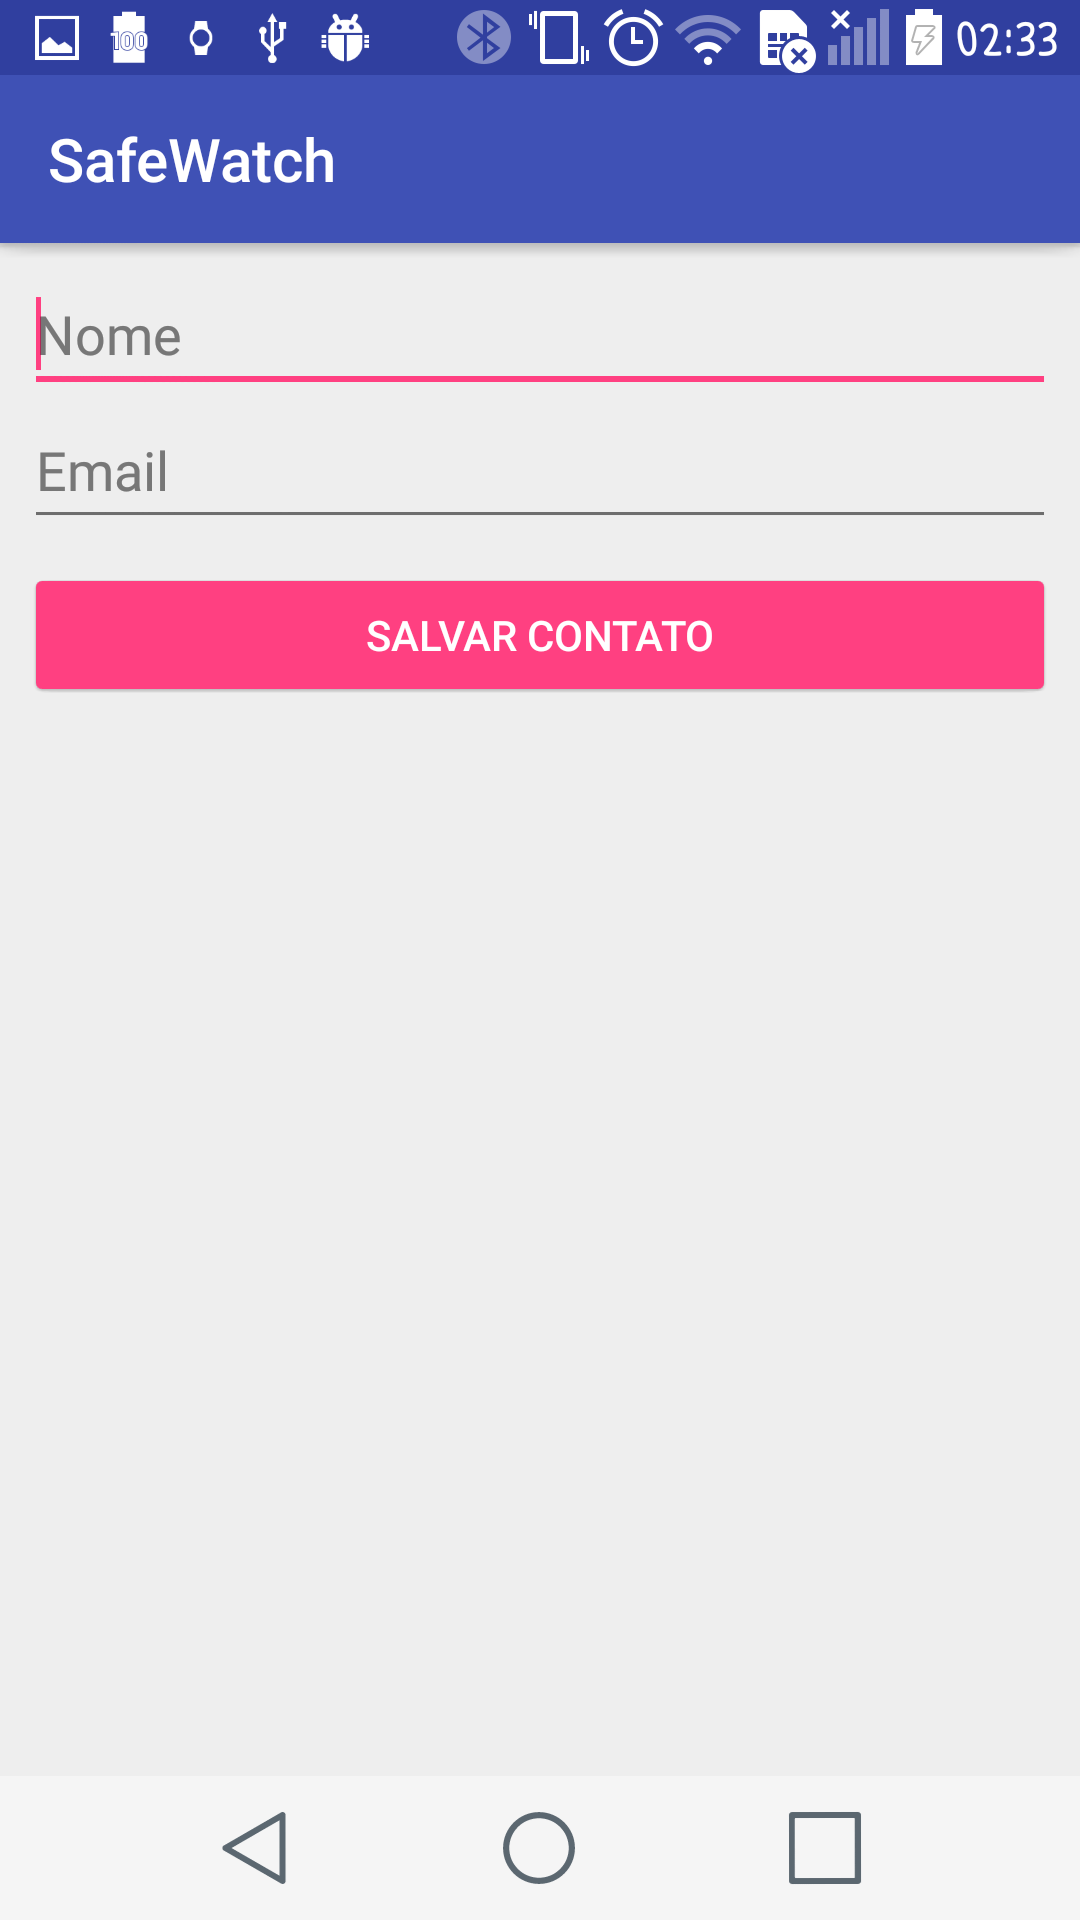
\includegraphics[scale=0.3]{imagens/tela_adicionar_contatos.png}
	\caption{Tela de adição de um contato de emergência. Figura Elaborada pelo autor (2016).}
	\label{fig:add_contact}
\end{figure} 


\begin{figure}[ht]
	\centering
	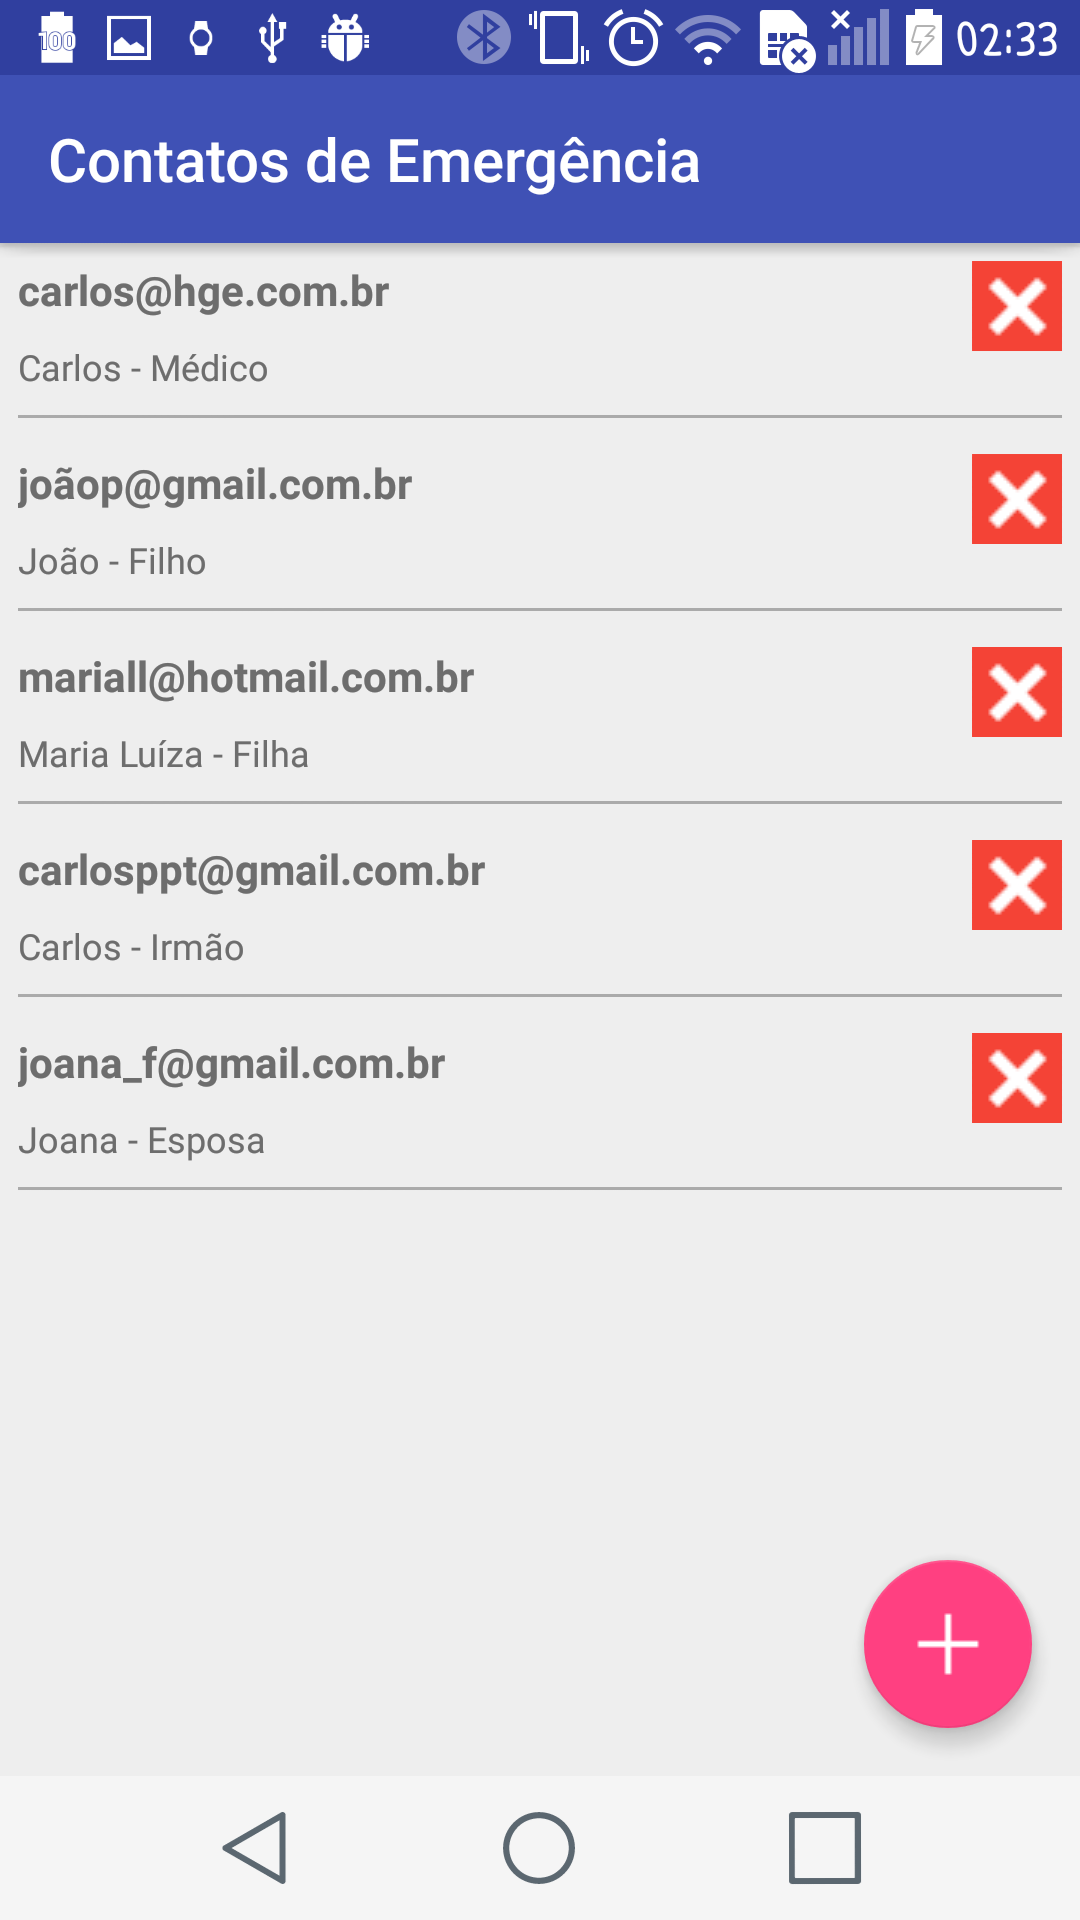
\includegraphics[scale=0.3]{imagens/tela_contatos.png}
	\caption{Tela de visualização dos contatos de emergência. Figura Elaborada pelo autor (2016).}
	\label{fig:list_contacts}
\end{figure}


\begin{figure}[ht]
	\centering
	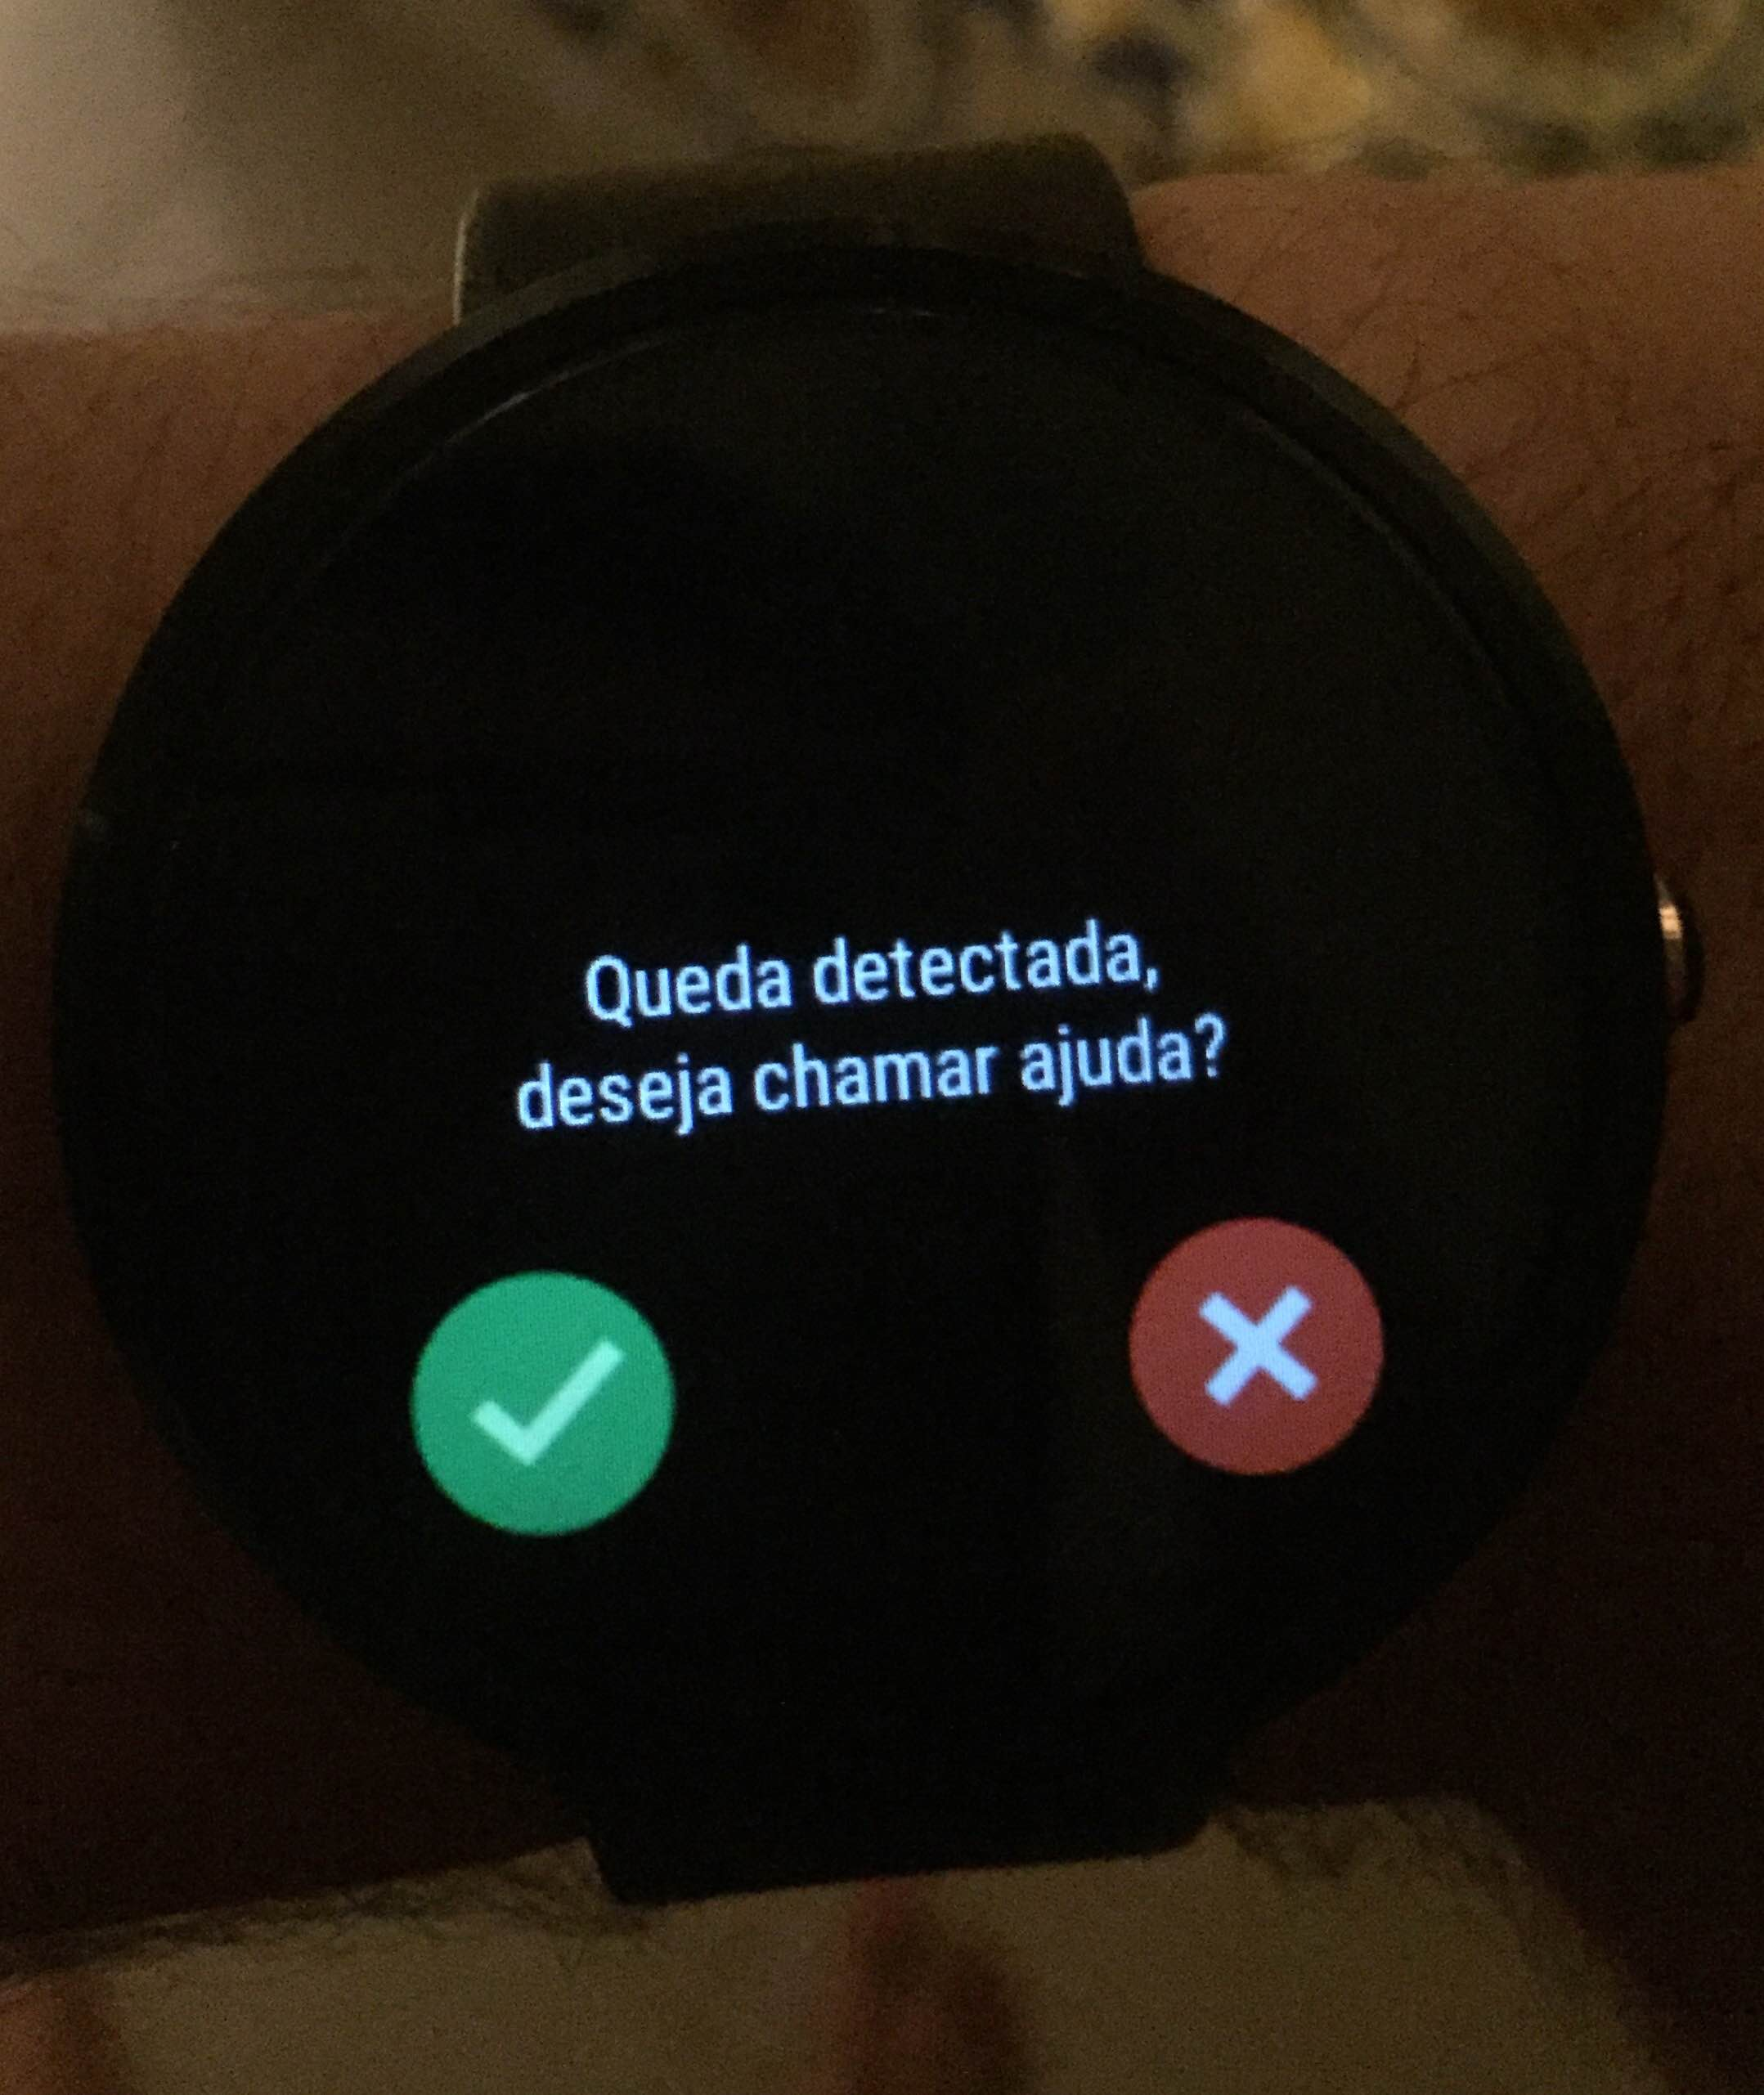
\includegraphics[scale=0.12]{imagens/screen_fall.png}
	\caption{ Tela apresentada quando uma queda é detectada. Figura Elaborada pelo autor (2016).}
	\label{fig:monitor_fall}
\end{figure}



\begin{figure}
	\centering
	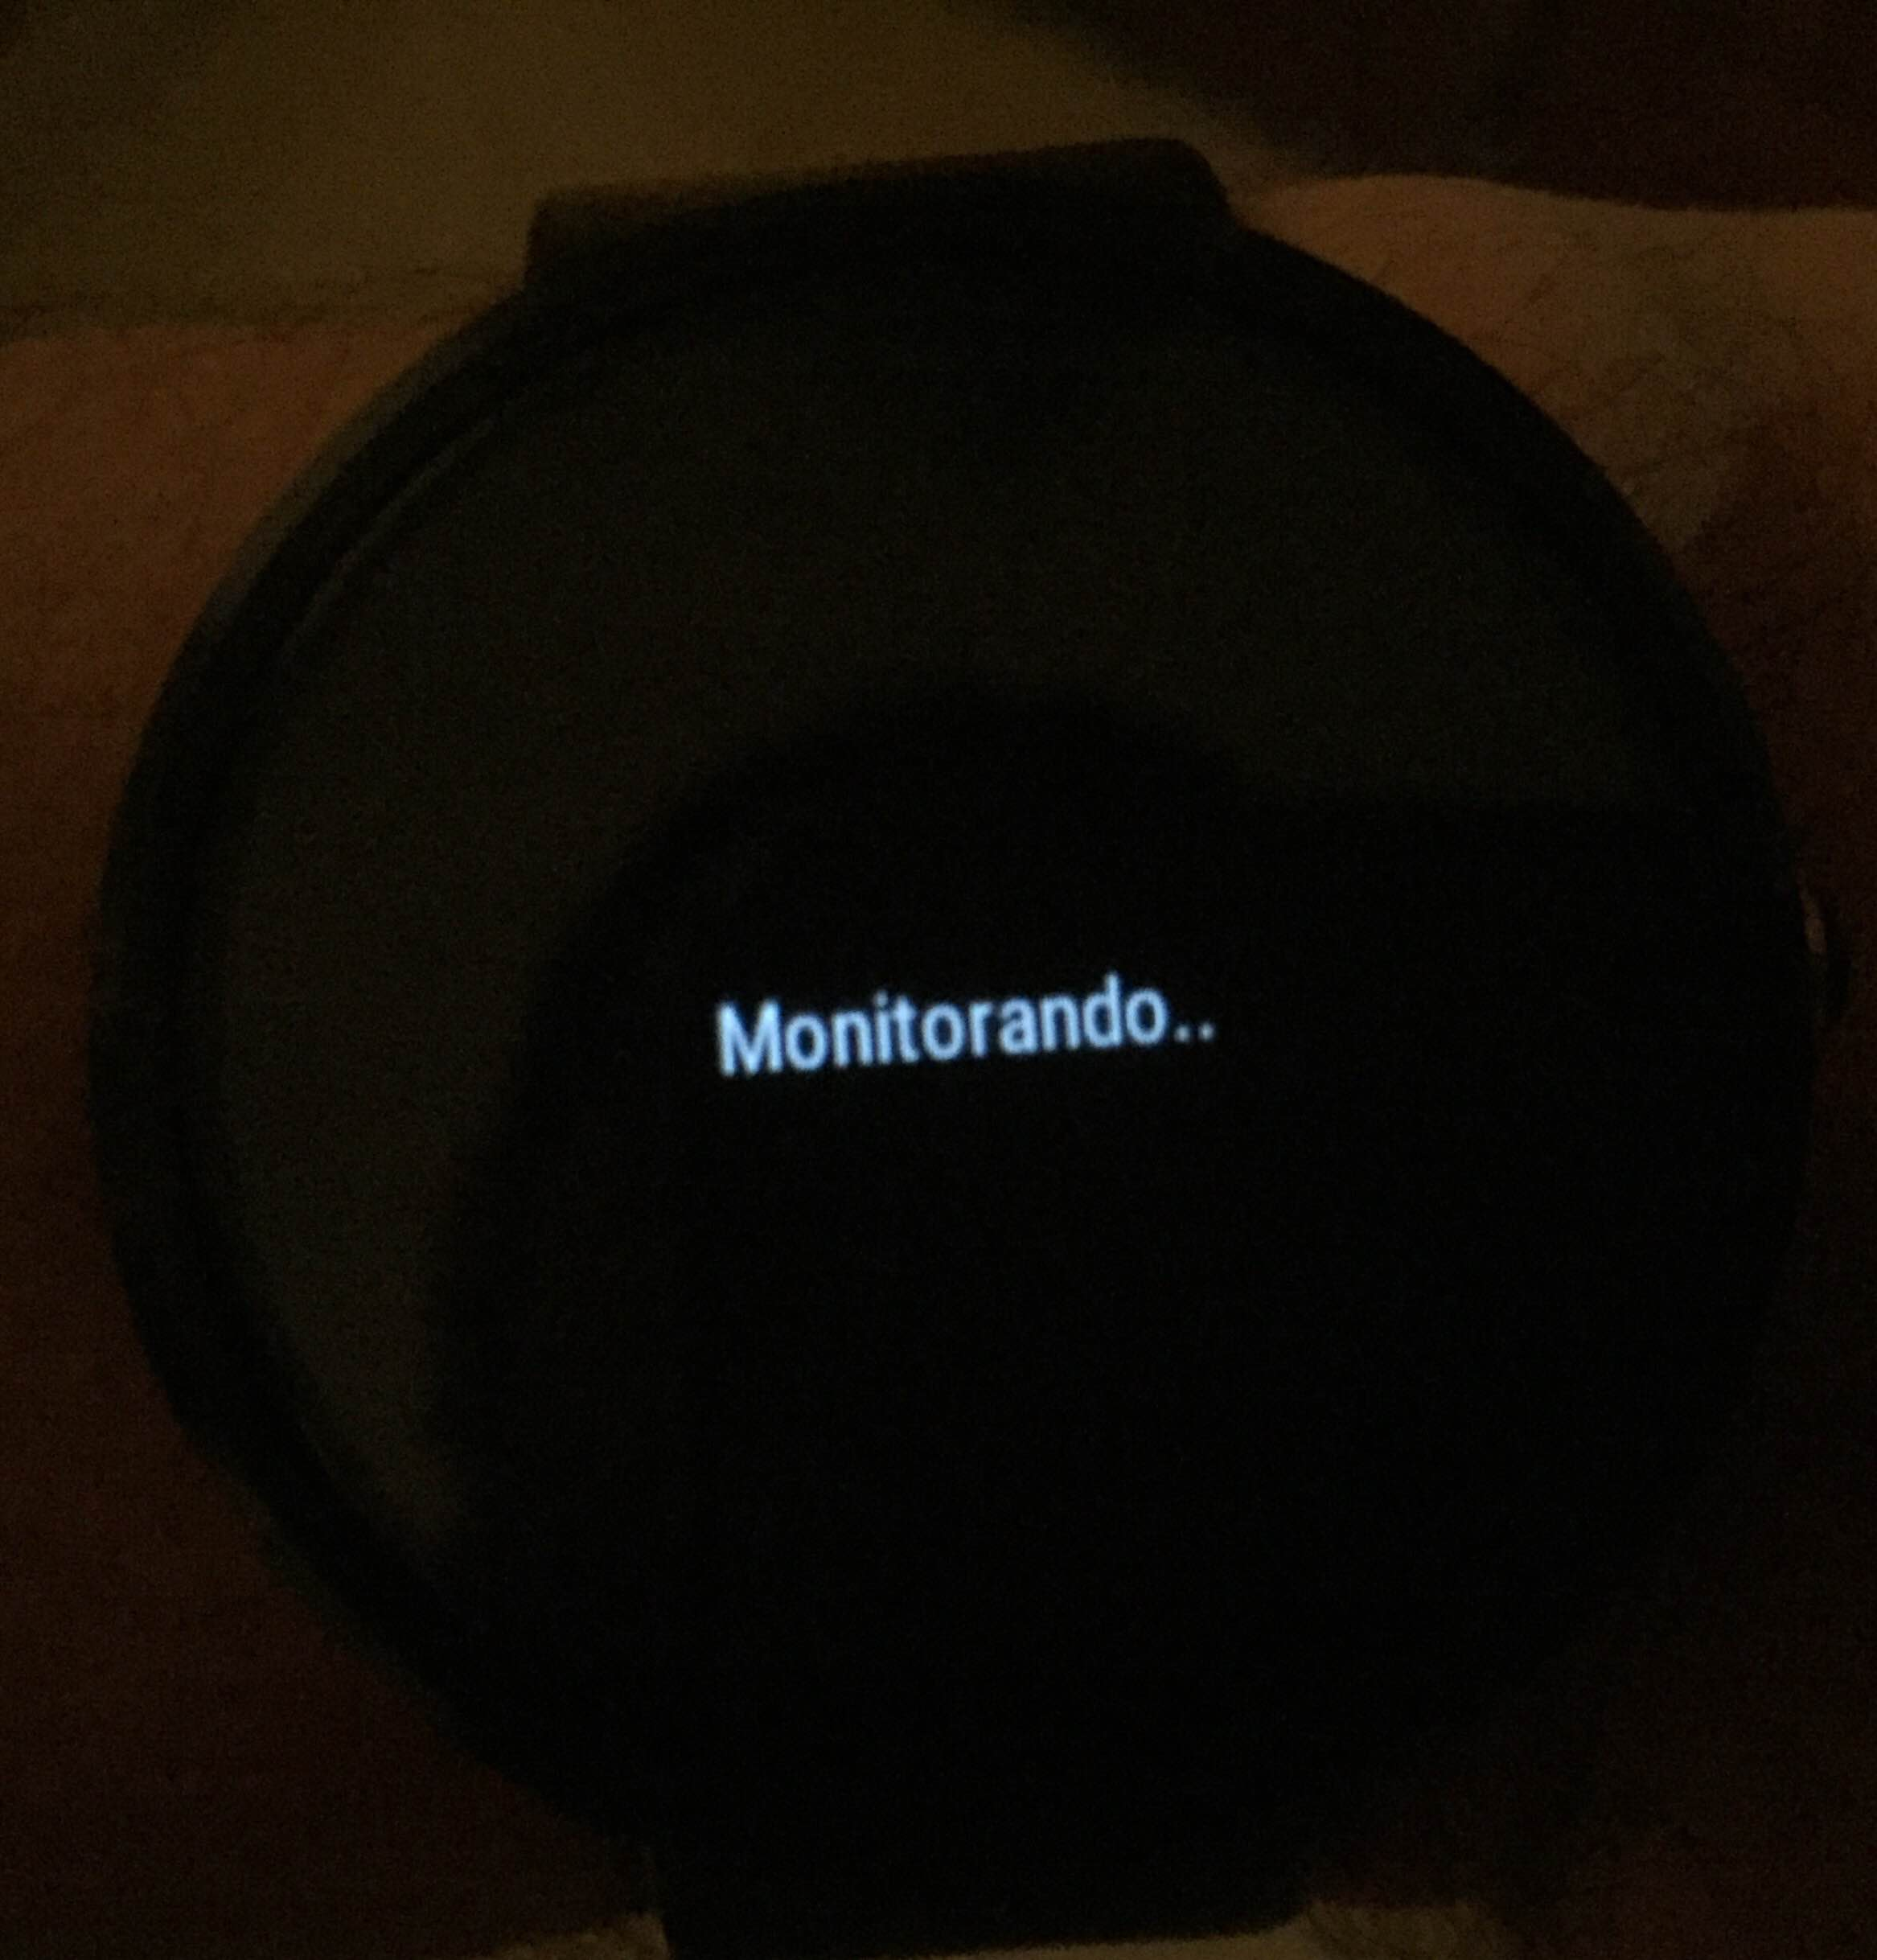
\includegraphics[scale=0.1]{imagens/screen_monitor.png}
	\caption{ Tela de monitoramento presente no smartwatch. Figura Elaborada pelo autor (2016).}
	\label{fig:monitor_screen}
\end{figure}


\begin{figure}[ht]
	\centering
	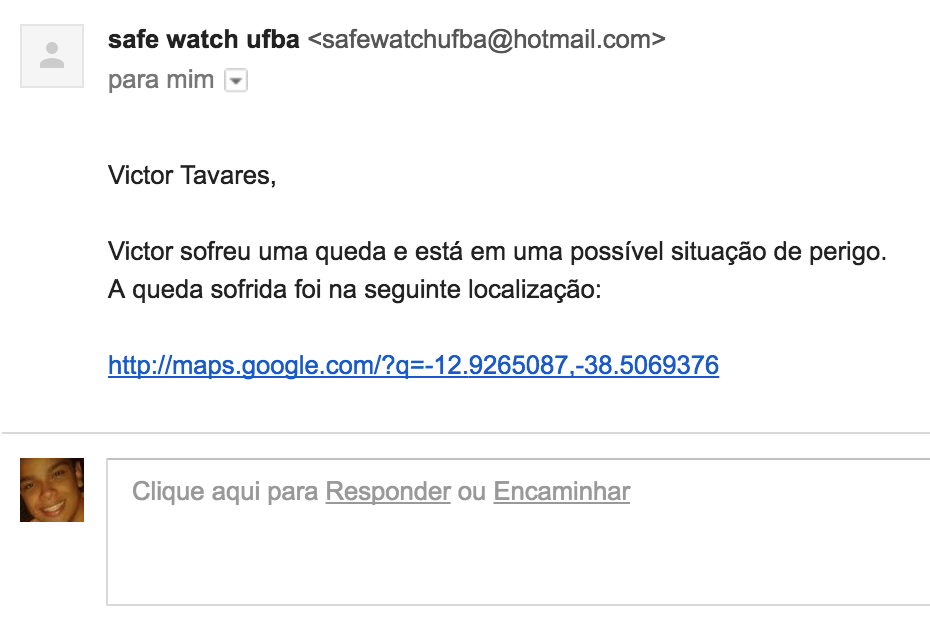
\includegraphics[scale=0.7]{imagens/mail_example.png}
	\caption{ Modelo de email enviado no evento de queda. Figura Elaborada pelo autor (2016).}
	\label{fig:mail_template}
\end{figure}

